\documentclass[sigconf]{acmart}

\usepackage{graphicx}
\usepackage{hyperref}
\usepackage{todonotes}

\usepackage{endfloat}
\renewcommand{\efloatseparator}{\mbox{}} % no new page between figures

\usepackage{booktabs} % For formal tables

\settopmatter{printacmref=false} % Removes citation information below abstract
\renewcommand\footnotetextcopyrightpermission[1]{} % removes footnote with conference information in first column
\pagestyle{plain} % removes running headers

\newcommand{\TODO}[1]{\todo[inline]{#1}}

\begin{document}
\title{Big Data Applications in Real Estate Analysis}


\author{Elena Kirzhner}
\affiliation{%
  \institution{Indiana University Bloomington}
  \streetaddress{3209 E 10th St}
  \city{Bloomington} 
  \state{Indiana} 
  \postcode{47408}
}
\email{ekirzhne@iu.edu}


\begin{abstract}

Big Data analysis reveals and comforts buyers with knowledge and facts about the neighborhood, its people and trends. Reducing risk of buying and predicting changes in home value for potential buyers.

\end{abstract}

\keywords{i523, hid320, Big Data Applications and Analytics, Real Estate}

\maketitle

\section{Introduction}

When one mentions American dream, home ownership is first aspect that comes to mind. Another part of the American dream is financial success and wealth building. Buying your dream home to raise the family is obvious part of the real estate.  For most Americans buying a home is the largest purchase they will ever make. Coupled with the fact that most conventional mortgages span 30 years research and analysis required to make educated choice should not be taken lightly as it will have implications on lifestyle for practically 40 percent of your lifetime.  Successful investment in your home, potential rental property or land can lead to financially windfall. Failure to make right choices in real-estate purchases may have disastrous consequences. Financial ruin is obvious part of the equation. Majority of divorces in the united states are caused by financial duress in the households. Resulting in stress negatively affecting one\textquotesingle s  health.

The latest trend in real estate is application of Big Data. Big Data manipulation is booming and transforming the industry. We are seeing a huge move in usage of Big data and analytics. Companies build property matching online software based on customers behavior and their needs. The opportunities of Big Data are truly endless. It creates the power to change our thinking in decision making and develops efficient business approach by extracting variety of collected data points and reducing risks for consumers.

Big Data is already changing real estate industry by optimizing consumers search, offers recommendations on real estate websites to potential buyers and sellers. Utilizing Big Data in real estate could match customers with their desired home. It might include how many bedrooms they need, what neighborhood fits best, affordability, schools, crime rates, potential business property for rent, location and communities.

When using Big Data and analytics, it is possible to review patterns to understand whether the property is a good investment and a great match to potential customer. It is also possible to analyze what buyers are selecting  more often and based on that data create a model.

When selecting a specific house for sale, Big Data integration within online websites made it possible to analyze local surroundings, sale patterns and neighborhood personality of each area. It created a knowledge comfort by having facts of the neighborhood, its people; and therefore reducing the risk of buying or investing in the wrong property. 

\section{Big Data in Real Estate Business}

Risk mitigation is essential part of the way Big Data is transforming real estate. Open data across the internet and variety of Big Data tools added strong force for analysis in decision making of choosing right property or home. It equipped customers with the valuable information by extracting the data and cross analyzing it.

Big real estate agencies such as Realtor \cite{realtor}, Zillow \cite{zillow} and Trulia \cite{trulia}, are pioneering those tools and provide estimated forecast of the property value from 1 to 10 years. Additionally, they provide information about the neighborhood trends, estimate mortgage payment, cost of ownership, history of the property and current value. The calculation is based on variety of public data records, market information, user data points \cite{zestimate} by using Big Data analysis formula developed in-house.

\subsection{Real Estate Industry Evolution}

Automated valuation methods have been used for a very long time. For decades banks utilized ''Automated Valuation Model'' to estimate home values. At one point banks wanted to exclusively rely on this model more than home values provided by professional appraisers. That practice led to problems with by omitting important nuances about condition resulting in overvaluation and undervaluation of properties. Big Data analysis and property estimates generated by online real estate giants are the next step in the evolution of real estate industry. This evolution diminishes importance and need for a real-estate agents as it is able to gather a lot of tribal information known only to experts in the area. That means this change can impact job market for over six hundred thousand active agents in the US.

\subsection{Real Estate and Artificial Intelligence}

Real estate businesses worry that unlocking the vast amount of data about properties could transform the business to be powered by artificial intelligence.   

However, based on the GeekWire article \cite{robots} big data and artificial intelligence will not replace real estate agents. Robots are just big help and enrichment to the business. It created much better and safer decision making models. Artificial intelligence will help to deliver information about real estate transactions and trends to consumers. 
It says that in future Amazon voice or Siri could provide useful information about popular housing trends and market value. Additionally, it can reveal the data on how many people were interested in the property and bids. 

So far it is not a robot that is thinking and proactively making decision, it is just a voice based system that extracts the information from Big Data. 

For the last twenty years, industry worries about loosing jobs in that area. However, the industry stayed the same.
People still want an advice before making an important decision. Even thought, there so much more information and streamlined sales, individuals that want relationships, empathy and connecting with people are still there.

Obviously, there is some fear in real estate that robots can rock the world for real estate business. However, Big Data empowers agents with information and data, it is making them better providers with higher service. 

\subsection{Online Real Estate Agencies}

Online real estate agencies calculate market value by using proprietary formulas. They are not providing expert estimation but a starting point in estimated property monetary worth. It is calculated from public data and surveys, by utilizing special features, market conditions and location. Additionally, they encourage consumers and homeowners to expand online data by doing other investigations such as comparing market prices for around areas, working with a real estate agent, getting an appraisal from an expert and visiting the house \cite{zestimate}.

For example Zillow, developed a Zestimate prediction\cite{zestimate}, which is Zillow\textquotesingle s estimate of a home that currently on sale, one to ten years from now. The provided information based on current house and market condition. Other real estate agencies with online presence competing with Zillow, like Trulia and Realtor for example have developed similar proprietary formulas to assist customers.

Also, the companies provide rent estimates that would help evaluate potential monthly rental price by developed in-house algorithmic formula. Variations in rental prices can also happen because of different factors, additional investments, or length of lease.

Big Data information affects the forecasting. As an example, the amount of rental listings in a specific area affects how much we know about approximate prices in that area for condos, apartments and houses. Based on number of properties for rent, the prediction becomes more accurate.  Homeowners can also update and provide information online about their needs or property, which helps even more for predicted accuracy.

The formula they use to estimate rent prices is comparing similar homes and apartments in the given area. Comparing bedrooms, square footage and other details. Then prices are being compared, and pattern to rental prices is shown.

Big data analysis provides unbiased information.  Although, majority of real estate agents are esteemed professionals looking out for client’s best interests they are still. There are still those that would like to manipulate client’s opinion to benefit themselves. For example, if a particular house have been on the market too long and the agent might lose the listing there is a possibility that some shortcoming of the property will be omitted by the agent in order to complete the sale. Same can be said about agents trying to achieve some sales goals or quotas. However, if the potential buyer conducts the research using Big Data all information will be available. Put simply, data does not lie.

\section{Real Estate Analysis}

Big Data is widely used by agents and real estate agencies to understand and improve how to target potential buyers. But the great thing about Big Data is that customers benefit from it as well. They can use free public resources with tons of data and information maps with different data analyzing tool options.

Latest tools allow to utilize Python to cross mix and match different values and data sets to analyze complex data. Prior to having these tools available such analysis would be an impossible task for individual users and required immense human and computing effort to complete. It is possible to visualize it by rendering correlations and trends. It reveals stunning insights in to chosen property for rent, business or home. 

There is so much information that it is important to understand which data is relevant to consumers and improves decision making. It is useful to analyze the data-sets when considering investing \cite{investopia}. The analysis can provide variety information and make the educated decision on the investment.

\subsection{Big Data Tools}

Analysis of these featured data points could be done with Python tool sets and libraries.

Python is a great programming language with variety of options. It is object oriented, semantically structured and great for scripting programs as well as connecting other programmable components. Python is considerably easy to learn and because of its high productivity and also became one of the favorite tools for programmers and data scientists. It contains libraries that are script importable and usable for a lot of use cases, such as image modification, scientific data analysis and server automation. Python world has been around for thirty years and a lot of code was written with multiple contributors. Variety of options built up on how to visualize the data \cite{van2011python}.

The most common type of visualization is a simple bar chart and line graph \cite{robbins2012creating}. It is popular and commonly used type of visualization to make comparison between values and variety of categories. It can be vertically or horizontally oriented by adjusting x and y axes, depending on what kind of information or categories the chart requires to  present. Parameters need to be identified, such as axes, similarities, title and decided on what exactly the visualization supposed to show.

To make a simple bar chart, a number some of the most popular tools and libraries that have been invented for plotting the data could be utilized. These include the most used and common tools such as: Pandas, Seaborn, Bokeh,  Pygal and Ploty.

Additionally, just like any other programming language issues, errors or questions with the libraries can be found on stack overflow page by Google search.

\subsection{Data Analysis}

For the purpose of this project, bar chart and graphs visualization methods with pandas modules in Python have been rendered and explained.
The simple form of this plot looks acceptable and easy to read. 

The techniques were done within Jupiter notebook \cite{md}. 

Jupiter notebook is great for running data sets analysis and for calculation projects. Jupiter notebook documents are readable files having the analysis description and the results in figures and tables as well as exportable files which can be executed to perform data analysis. It allows to render images and move values back and forth between different modules and coding languages.

The data-sets collected from clrsearch.com \cite{clr}, data.gov \cite{data.gov}, zillow.com \cite{zillow} and uploaded to the class\textquotesingle s Google Drive to demonstrate the trends and patterns between each output. 

The data includes both geographic and social data-sets evaluated by ratings in rows and titles in columns to keep it simple. The data set for both cities is being used for all examples that are demonstrated below. 
The point of the visualization is to understand the data in visual platform and make an informative decision based on rendered data.

A simple example of two properties in Tarzana, California versus Calabasas, were compared and exported for read. 

Tarzana City is a wealthy neighborhood in the San Fernando Valley region of the city of Los Angeles, California. Tarzana was purchased in 1919 and developed on the site of local elites and named by Edgar Rice Burroughs, author of the popular Tarzan books. He established Tarzana and later sold it to local farmers \cite{wiki}.

Calabasas City located in the hills west of Malibu, in the San Fernando Valley region of the city of Los Angeles, California. The area established in 1991 and the name was derived from Spanish word ''calabaza'', meaning pumpkin.The legend has it that in 1824, a Mexican rancher spilled a wagon of pumpkin seeds and it spouted alongside the road. Therefore, the area was named Calabasas, the pumpkin land \cite{wiki}.

From a quick glance both areas are very similar and are located within 10 miles of each other. Both Tarzana and Calabasas are influential and desirable neighborhoods with lots of high priced homes. How does one differentiate between the two in order to find the right investment?

Big Data is the answer. Specifically in states like California.  In California Big Data application benefits greatly from availability of public records such as sale price as apposed to certain ''non-disclosure'' states. There sale prices for homes are not disclosed in public records.

The analysis combines several main components, including property characteristics in the area, crime rate, quality of life, pollution, race and ethnicity, population growth, family household, house value, business field, employment, schools and future home value.

\subsection{Property Characteristics}

Big Data analytics can help in connecting needs of a buyer and providing neighborhood demographics. The quality of population in the neighborhood will influence who buys the house and who lives there. It is important to identify what is important to you and make sure those items are covered in the research.  For example, if you are a student you will probably look for a densely populated location around universities, closer to food locations and communities. Things like public transportation,nightlife, and bars will be very important to you and will be prioritized over other things. If you are married with kids, your best choice would be location with good schools and low crime. Parks, playgrounds and traffic and noise pollution around the house will be paramount. Most parents would love to find a nice quite cul-de-sac house. Young working professional would prefer to be right in the middle of things on a busy boulevard.  

Latest Big Data collections made it all possible for real estate website to provide that information to potential buyers. Websites such as United States Zip-codes \cite{zipcodes} collect information from public records and make it available in exportable format as well as for reviewing and analyzing local neighborhoods by states and zip codes input. 

\subsection{Crime Rate Indexes}

Crime Big Data is available now and helps to see patterns and avoid areas with unfavorable statistics. The Los Angeles Police Department \cite{federal} already uses the data to show which areas in Los Angeles are hot-spots of crime.

Crime rates are being calculated by comparing the national levels of the average 100 \cite{crime}. For example, if score is 150 it means that it is 1.5 higher risk of crime that national average level. The data is coming from police department reports and public records. Additionally, the Federal Bureau of Investigation also provides factual information for ranking \cite{crime2}. Furthermore, the research on crime can be extracted from United States Department of Justice via Uniform Crime Reporting Program  \cite{unicrime}.

In this example \cite{md}, running the crime data sets of Tarzana and Calabasas showed that Calabasas is in much better shape and safer place to live as compared to Tarzana, which is around the average of national rate. The total crime risk in Tarzana slightly higher than national average, it is 108, meanwhile Calabasas is almost 3 times lower, it is 24. The murder risk is 118 compared to 24 in Calabasas. Rape risk is 70 in Tarzana and 35 in Calabasas. Robbery risk in Tarzana is almost twice higher than in Calabasas, it is 125 versus 77. Assault risk three times higher in Tarzana, it is 127 versus 48 in Calabasas. Burglary risk twice higher in Tarzana as well, it is 55 versus 27. Larceny risk in Tarzana is overwhelmingly high, it is 73 versus 9 in Calabasas. Motor vehicle theft risk in Tarzana is 118 versus 39 in Calabasas. Based on these findings, it is defiantly safer to live in Calabasas [fig 1].

Based on these finding, it is defiantly safer to live in Calabasas as shown in Figure \ref{fig:figure1} \cite{md}.

\begin{figure}
  \centering
  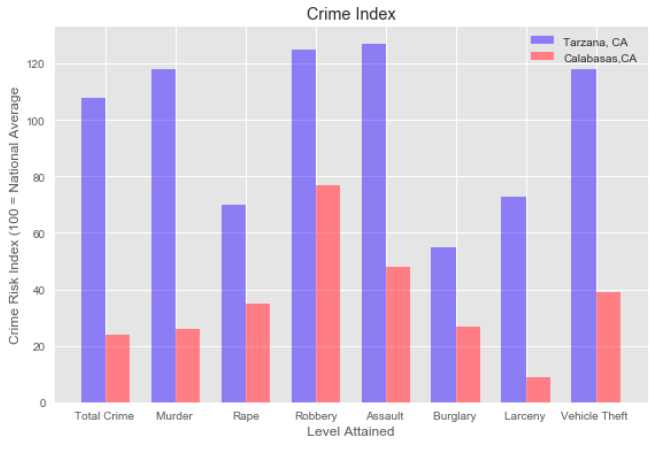
\includegraphics[width=0.5\textwidth]{images/figure1.png}
  \caption{Crime rate in Tarzana, CA compared to Calabasas, CA (100 = National Average) \cite{md}.} \label{fig:figure1} 
\end{figure}

\subsection{Education Levels}

Next run was done on educational level of residents.
Big Data includes data of resident\textquotesingle s education level and makes it possible to collect data about an individual resident and provides insightful information about social level interaction. The data extracted and combined from variety of sources including international school districts. 

The education rating  filtered by zip codes represents the percentage of people in the area who have attended colleges and received degrees. It does not represent performance and specific schools. 

The rendered data showed \cite{md} that residents in Calabasas are higher educated by 7 percent with Bachelor degrees and 6 percent higher with graduate degree, as shown in Figure \ref{fig:figure2} \cite{md}.

\begin{figure}
  \centering
  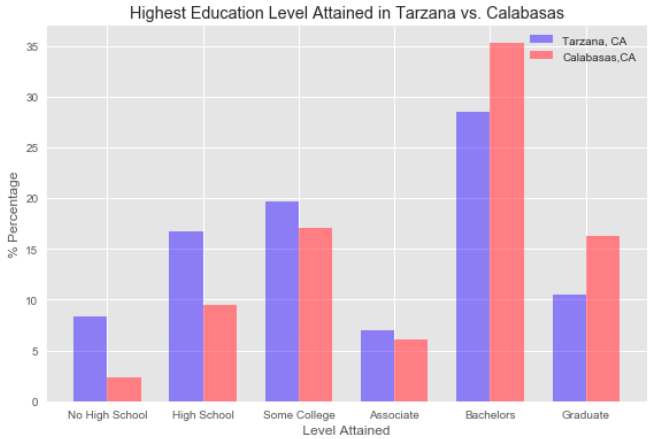
\includegraphics[width=0.5\textwidth]{images/figure2.png}
  \caption{Educational percentage of people in Tarzana, CA compared to Calabasas, CA (Population Age 25+) \cite{md}.} \label{fig:figure2} 
\end{figure}

Based on the Economic Policy Institute study \cite{education}, there is a clear correlation between higher educated workforce and economic success within state and ability to grow. Additionally, higher educated people are good for state budgets, since workers with higher income contribute more through taxes. 

\subsection{Life Quality Standards}

The next important consideration in buying a property, searching for a house and making a decision is quality of life standards in that area. Big Data and and latest methods of data collection can lead to improvements in quality of life for residential areas. It can find neighborhoods that are safer, cleaner, more entertaining and a better place to live specifically tailored to potential buyer. 

The data-set of life quality obtained from variety of sources, including public Google searches, social media and local study groups. The quality of life is being measured by how residents are being effected by crimes, weather, education, entertainment, religion, medical support and food supply.    
The positive decision variables calculated by amusement, education, culture, media, religion, weather and restaurants. The negative decision is based on the level of crime, natural disasters and mortality. The  national level is being compared to 100 \cite{clr}.   

Rendered data showed that amusement index equal to 110 in Tarzana and 130 in Calabasas. What that means is that in Calabasas there are more community events and entertainment. Culture is 142 in Tarzana versus 129 in Calabasas. Culture refers to artistic development. Earthquake index 362 in Tarzna compared to 318 in Calabasas. this is a very intresting point considering that both neighborhoods are very close to each other. But since Tarzana's Earthquake index is higher associated insurance will likely be higher as well.  Raising cost of ownership. Medical index is 137 in Tarzana and 116 in Calabasas.If you are working the the medical field this might be an important topic for you as it will help you find employment closer to home. Reduce your commute time, minimizing wasted time spent in California's infamous gridlock traffic. Mortality is much higher in Tarzana, it is 144 versus 95 in Calabasas. Religion is better in Tarzana, it is 154 compared to 96 in Calabasas. Religion refers to houses of worship and religious establishments. Restaurant index about the same, it is 144 in Tarazana and 139 in Calabasas. Weather is better in Tarzana, it is 16 versus 10 in Calabasas. That is another interesting observation considering that both neighborhoods are minutes away from each other.

Based on the data, overall quality of life is equal between two cities, as shown in Figure \ref{fig:figure3} \cite{md}.

\begin{figure}
  \centering
  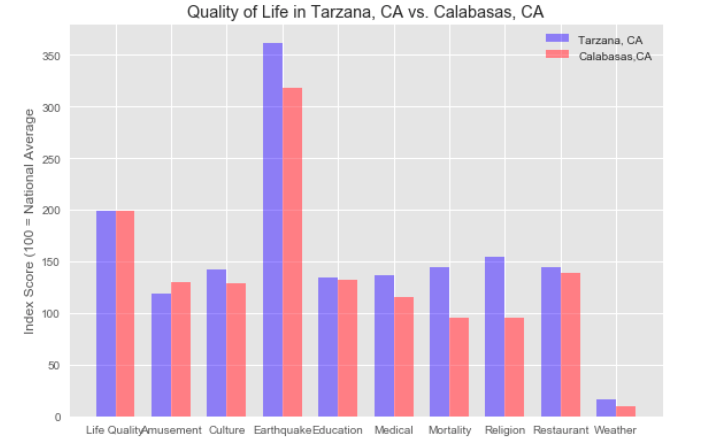
\includegraphics[width=0.5\textwidth]{images/figure3.png}
  \caption{Life quality of people in Tarzana, CA compared to Calabasas, CA  \cite{md}.} \label{fig:figure3} 
\end{figure}

\subsection{Air Pollution}

Big data can control and reveal pollution levels of particular area \cite{pollution}. It is one of the main causes of health problems in the population and preventive cause death.

Over 80 percent of residents living in urban areas are vulnerable to poisoning from pollution.  Cancer is one of the leading cause of deaths for both men and women; and exposure to pollution at early may have life-long negative consequences.  

Monitored areas show that air quality levels exceed the safety levels \cite{pollution2}. Additionally, the World Health Organization warns that most populated states are most affected.

Government is aware of this problem, therefore collecting and monitoring the data regarding air quality has increased. The data is being shared between universities and air quality maps for further development. The data is openly shared and prepared for Big Data analysis.

Even thought Big Data will not reduce the pollution by itself, it provides tools to visualize the problem which is especially helpful when choosing a place to live.

The exported data-sets showed \cite{md} that carbon monoxide is extremely high in both cities. It is 186 in Tarzana and 183 in Calabasas. The national level is being compared to 100 \cite{clr}. Based on the data, overall air pollution index is about the same in both areas, as shown in Figure \ref{fig:figure4} \cite{md}.

\begin{figure}
  \centering
  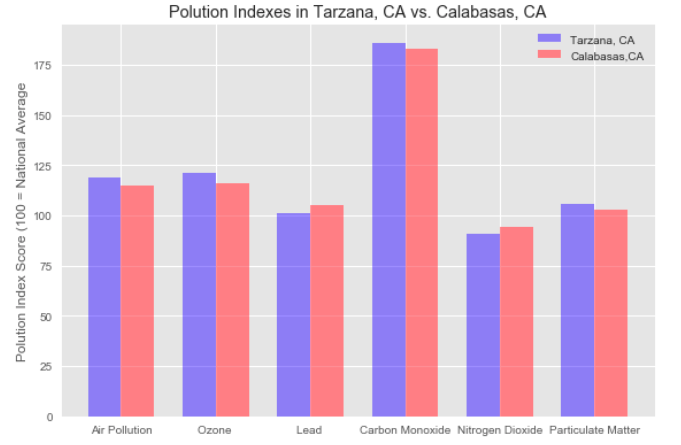
\includegraphics[width=0.5\textwidth]{images/figure4.png}
  \caption{Air Pollution Indexes in Tarzana, CA compared to Calabasas, CA \cite{md}.} \label{fig:figure4} 
\end{figure}

\subsection{Race and Ethnicity}

Big Data can reveal a lot of information about population by using zip codes. It shows profiles of people who live there. 
Understanding ethnicity and identity of the community influence will help with decision.

The standard of maintaining, collecting and presenting federal data on race and ethnicity \cite{race} were revised and improved on collecting quality about two decades ago. In accordance to best analysis practices, federal agencies conducting researches to better understand ethnic and race diversity.

The language to describe the ethnicity and race keeps changing to resonate with the category of residence and adding new meaning to not make it discriminatory.  The general rule became that race and ethnicity should not be interpreted as being a science. 

Based on the rendered graph, most population in Tarzana and Calabasas consist of white and non-Hispanic residents, as shown in Figure \ref{fig:figure5} \cite{md}.

\begin{figure}
  \centering
  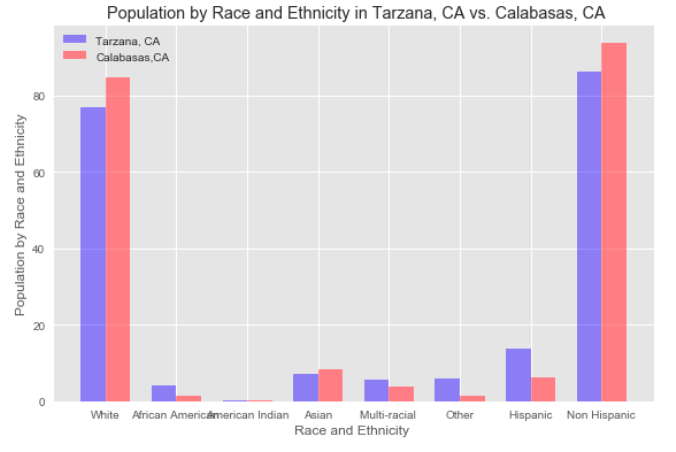
\includegraphics[width=0.5\textwidth]{images/figure5.png}
  \caption{2012 Population by Race and Ethnicity in Tarzana, CA compared to Calabasas, CA \cite{md}.} \label{fig:figure5} 
\end{figure}

That information provides insight about communities and relatedness to the buyer.

\subsection{Population Growth}

Leveraging Big Data in population growth might be helpful for economic growth prediction and future development.

For the recent centuries, population growth jumped dramatically \cite{population}. How fast the population is growing can influence area homes and businesses development. Allowing for more business opportunities.   

Educated people can contribute to the development with increased skills and knowledge. However, it is also important to look not only on the total population size, but also population growth rate.

Based on the data visualization, population size in Tarzana is higher by 3,000 residents than in Calabasas, as shown in Figure \ref{fig:figure6} \cite{md}.

\begin{figure}
  \centering
  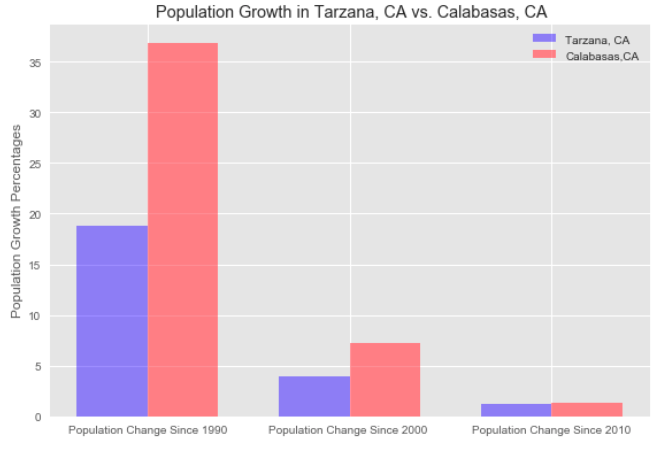
\includegraphics[width=0.5\textwidth]{images/figure6.png}
  \caption{Population change since 1990 in Tarzana, CA compared to Calabasas, CA  \cite{md}.} \label{fig:figure6} 
\end{figure}

Both in Calabasas and Tarzana, the rate was rapidly increasing from 1900-2000, and there was not much progress since then. Population density in Tarzana is  4,048 versus 856 in Tarzana. City area size in square miles is 7.44 and 31.67 in Calabasas. 
This information provides insight that Calabasas has much more opportunities for future growth and development. New housing and real estate development is achilies heel in California.  State struggles to provide all existing residents with affordable housing. Compiled with population growth and migration of new residents the problem becomes even harder resolve.  By having additional development space  Calabasas growth potential is much higher compared to Tarzana.

\subsection{Family Household}

Big Data and internet of things are making its existence common place in each household. Only 15 years ago home computers were the only smart device in the house.  Now even vacuums and thermostats are connected. Our homes are goldmines of data.  Getting family household data summary instantly tells about the type of people in these areas and obtained knowledge can be used to help with buying decision.

Household definition refers to type of family and people living in a household structure.
Household data is useful when consumer wants to know about the type of people living in that area and relativity.

Based on the combined data-set results \cite{md}, full family household is 64 percent in Tarzana and 76 percent in Calabasas. 48 percent are married in Tarzana, and 62 percent in Calabasas. Therefore for married families with kids it makes more sense to live in Calabasas.

\subsection{Property Value}

Big Data is being used to analyze property values. Real estate agencies, such as Zillow \cite{zillow}, estimate values based on Big Data collection tools and using their algorithm  \cite{zestimate}.They combine information from variety of sources and provide insightful information to buyers, sellers or brokers. 

Based on the data analysis \cite{md}, it shows that Calabasas prices are higher than in Tarzana by 23 percent. That insight shows that more financially able residence live in Calabasas.

To confirm that, the income data was calculated. Based on the rendered data as shown in Figure \ref{fig:figure7} \cite{md}, it proves that residence in Calabasas are more influential with higher income than in Tarzana.

The total income in Calabasas is higher by approximately 20 percent.

\begin{figure}
  \centering
  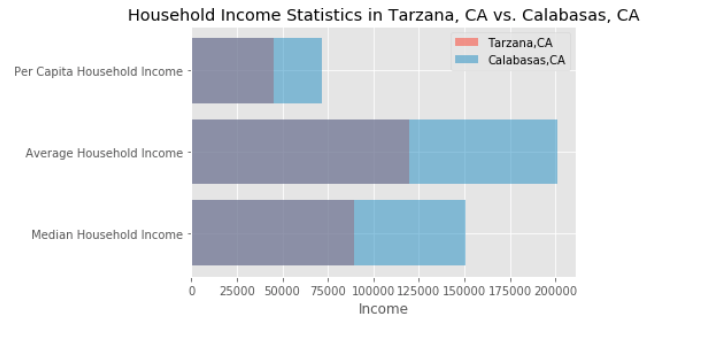
\includegraphics[width=0.5\textwidth]{images/figure7.png}
  \caption{Income in Tarzana, CA compared to Calabasas, CA  \cite{md}.} \label{fig:figure7} 
\end{figure}

\subsection{Employment and Occupation}

The employment breakdown that derived from data, published by the Bureau of Labor Statistics showed that business field compared with employment field could help with predicting job opportunities.

Based on compared data sets, Health-care is leading employment field in Tarzana and Managment in Calabasas, as shown in Figure \ref{fig:figure8} and Figure \ref{fig:figure9} \cite{md}.

\begin{figure}
  \centering
  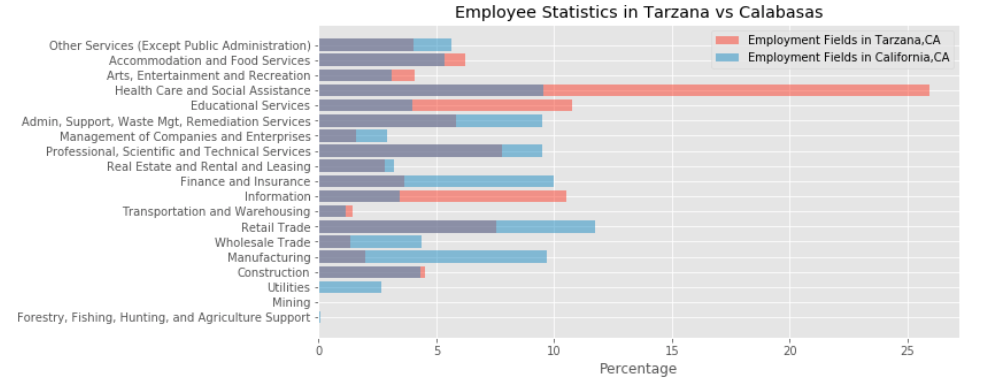
\includegraphics[width=0.5\textwidth]{images/figure8.png}
  \caption{Employment field in Tarzana, CA compared to Calabasas, CA \cite{md}.} \label{fig:figure8} 
\end{figure}

\begin{figure}
  \centering
  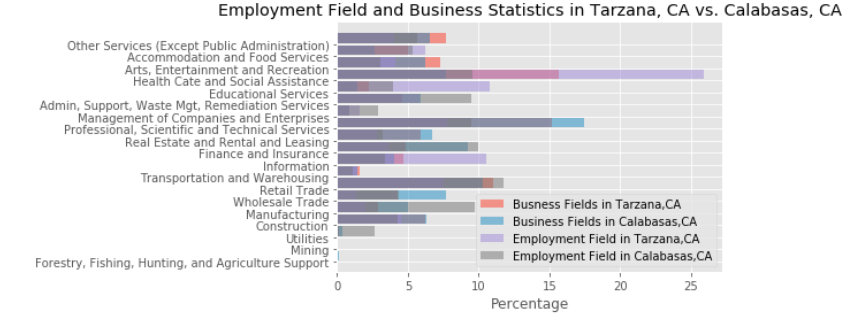
\includegraphics[width=0.5\textwidth]{images/figure9.png}
  \caption{Business fields in Tarzana, CA compared to Calabasas, CA \cite{md}.} \label{fig:figure9} 
\end{figure}

\subsection{Public Schools}

Big Data in public schools are being used to fix education institutions and improve student scores and results. whereas in the past school performance was judged simply on average API scores of the students now student attributes data is further analyzed.  This allows to identify subgroups of under-performing students.  For example income levels of households are tracked to make sure that students from low-income families have the same opportunities to have better scores and grades as families from high-income families. It also provides tracking and comparison with schools in different districts. This helps school boards to allocate additional resources to schools that lack them.  It also helps parents and home buyers identify schools and neighborhoods where their child could flourish academically.   

The mined data could be used for decision making in property investment as well. Prospective buyers with kids are not only looking for good education and safe schools for their own kis, but also from stand-point of property value since homes located in good school districs are more desirable. The detailed information that can be found online made it easy to be properly informed. 
Compared data between two cities, showed that elementary schools have 38 percent higher rating in Calabasas, middle schools are 25 percent higher and high schools are the same. 
Schools in Calabasas are better based on these rating scores, as shown in Figure \ref{fig:figure10} \cite{md}.

\begin{figure}
  \centering
  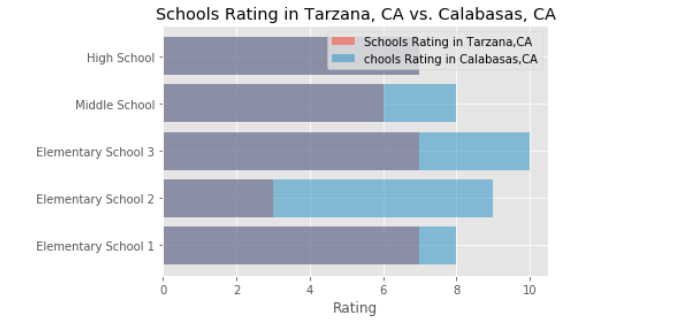
\includegraphics[width=0.5\textwidth]{images/figure10.png}
  \caption{Public schools in Tarzana, CA compared to Calabasas, CA \cite{md}.} \label{fig:figure10} 
\end{figure}

\subsection{Available Houses for Rent and Sale}

Another shift in demographic preferences that has been observed is related to home ownership vs renting.  Millenniums are changing their spending habits when compared to previous generations. Food, health and entertainment take priorities over burdens expenses associated with home ownership.  If that trend continues return on investment generated by buying rental properties will rise.

The best way to know if a house is a good investment is to check the rental properties near the area.

There is also a 1 percent rule of thumb to keep in mind. The rule is that a purchased home should be rented for 1 percent of the cost.

Based on the rental data, medium price in Tarzana 4,210 dollars per month, and Calabasas 4,085 dollars per month. It actually reveals that Tarzana rental properties are more expensive than Calabasas, even thought the home prices in Calabasas are higher, as shown in Figure \ref{fig:figure11} \cite{md}.

\begin{figure}
  \centering
  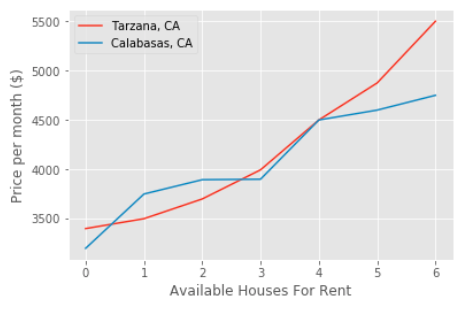
\includegraphics[width=0.5\textwidth]{images/figure11.png}
  \caption{Houses for rent in Tarzana, CA compared to Calabasas, CA (3bd+ House For Rent (1,500-2,500 Sqft)) \cite{md}.} \label{fig:figure11} 
\end{figure}

Additionally, square footage was calculated. To get the price per square footage, the price of the area was divided by its square footage. The results showed that in Tarzana rent is slightly higher than in Calabasas, as shown in Figure \ref{fig:figure12} \cite{md}.

\begin{figure}
  \centering
  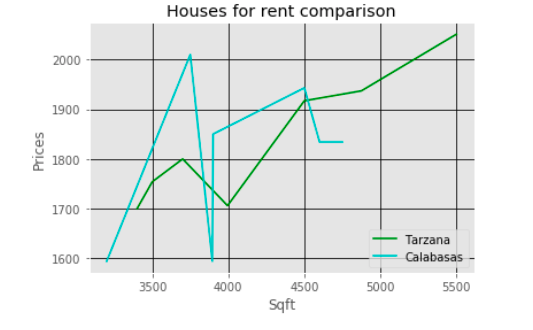
\includegraphics[width=0.5\textwidth]{images/figure12.png}
  \caption{Price per sqft for rent in Tarzana, CA compared to Calabasas, CA \cite{md}.} \label{fig:figure12} 
\end{figure}

Therefore, it makes more sense to buy renting properties in Tarzana.

The lowest price of property in Tarzana is 700,000 us dollars, and in Calabasas it is 975,000 us dollars \cite{md}.

Based on the 1 percent rule, it does not make sense to buy and rent out in Tarzana or Calabasas.

\subsection{Future Value}

California housing is booming and crashing. Massive home equity destruction happened few years ago and reversed back. 

When data-sets are analyzed, they can reveal insightful information and guide consumer decision making.

Based on the sales data was taken and generated, suggests that in spite of prices drops the value of houses goes up, as shown in Figure \ref{fig:figure13} and Figure \ref{fig:figure14} \cite{md}.

\begin{figure}
  \centering
  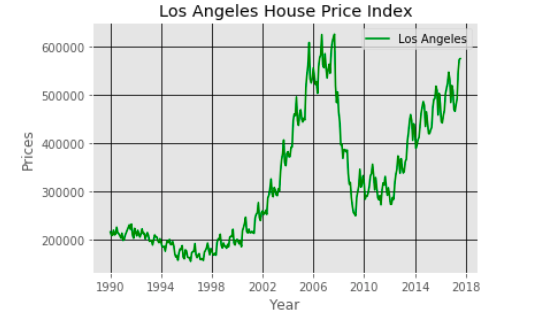
\includegraphics[width=0.5\textwidth]{images/figure13.png}
  \caption{Prices Growth Index in California \cite{md}.} \label{fig:figure13} 
\end{figure}

\begin{figure}
  \centering
  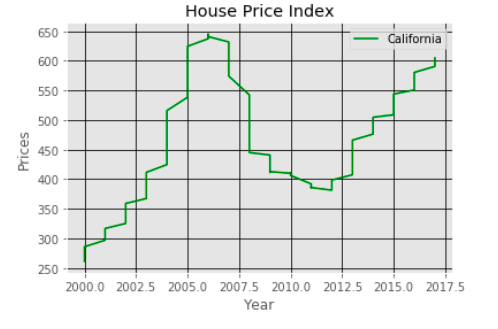
\includegraphics[width=0.5\textwidth]{images/figure14.png}
  \caption{Prices Growth Index in California \cite{md}.} \label{fig:figure14} 
\end{figure}

Calculated housing investment for the last 20 years had a growth rate of 5.46 percent \cite{md}. By knowing a starting and ending value, it is possible to calculate the future value of an investment. Referencing the previous calculations \cite{md}, it predicts that house value will grow by 63 percent in the next 20 years.

\section{Conclusion}

Big Data potential to transform decision making in real-estate is immense. Home ownership is part of the American dream and Big Data will play a huge role in that process. It will allow potential buyers to have a better understanding of historic data and how it correlates to investment potential.

Big data will provide powerful insight to augment decision making process. Yet, it will not eliminate all risks associated with investment in real-estate. All risks must be evaluated and analyzed before buying and big data will provide plenty of tools for that.

Based on this analysis, it was determined that Tarzana and Calabasas properties are overpriced. Currently, renting is low compared to buying a property.

It is impossible to find properties in California that generate rents at around 1 percent of total property cost. You can not justify the prices and it is only for the privilege of living in San Fernando Valley region of the city of Los Angeles, California.

However, if you do still want to invest, Calabasas is a better choice for investing in a family home property and Tarzana for a rental property.

\begin{acks}

  The author would like to thank Dr. Gregor von Laszewski, Juliette Zerick and Miao Jiang for their help, support and suggestions to write this paper.

\end{acks}

\bibliographystyle{ACM-Reference-Format}
\bibliography{report} 

\end{document}

